\documentclass[12pt]{article}

% Specify how big is going to be the paper margins.
\usepackage[a4paper, margin=1in]{geometry}

% amsmath: Add useful commans like aligh and gather.
% amsfonts: Add useful fonts like \mathbb{R}.
% amssymb: Add useful symbles like \therefore (needs amsfonts to work).
\usepackage{amsmath, amsfonts, amssymb}

% Makes the use of colors possible.
\usepackage{xcolor}

\definecolor{color1}{HTML}{0e4a7a}
\definecolor{color2}{HTML}{1282d6}
\definecolor{color3}{HTML}{7ac1ff}

% Add Latin Modern Fonts like Sans-serif and Roman.
\usepackage{lmodern}

% Makes header and footer configurable.
\usepackage{fancyhdr}

% Makes the use of colored and configured tables possible
\usepackage[most]{tcolorbox}

% Add commands to specify theorems like \newtheorem{x}{y}.
\usepackage{amsthm}

% Enables enumeration of items.
\usepackage{enumitem}

% Enables adding images.
\usepackage{graphicx}

% Enables cool hyper references.
\usepackage[colorlinks=true, linkcolor=color2, urlcolor=color2, citecolor=color2]{hyperref}

\title{\sffamily\bfseries{Soluções Jacob Palis 2022 N2}}
\author{Samuel de Araújo Brandão}
\date{4 de Setembro de 2025}

\pagestyle{fancy}
\fancyhf{}

\fancyhead[L]{\sffamily\bfseries{Soluções Jacob Palis 2022 N2}}
\fancyhead[R]{\textcolor{color2}{Samuel Brandão}, 4 de Setembro de 2025}
\fancyfoot[C]{\thepage}
\setlength{\headheight}{14.5pt}

\tcbset{
  statementbox/.style = {
    enhanced,
    width=\textwidth,
    title={Enunciado},
    title filled,
    fonttitle=\sffamily\bfseries,
    coltitle=white,
    colbacktitle=color1,
    colback=white,
    colframe=color1,
    boxrule=1pt,
    arc=2mm,
    boxsep=2pt,
  }
}

\tcbset{
  theorembox/.style = {
    enhanced,
    width=\textwidth,
    colback=white,
    colframe=color1,
    boxrule=1pt,
    arc=2mm,
    boxsep=2pt
  }
}

\tcbset{
  lemmabox/.style = {
    enhanced,
    width=\textwidth,
    colback=white,
    colframe=color2,
    boxrule=1pt,
    arc=2mm,
    boxsep=2pt
  }
}

\renewcommand*\contentsname{\textsf{Conteúdos}}
\newcommand{\kb}[1]{\left\lfloor #1 \right\rfloor}

\begin{document}
  \maketitle
  Uma coleção de soluções para a \textbf{Jacob Palis 2022 Nível 2}, inspirada no estilo de Evan Chen.
  Pode-se encontrar todos os problemas \textbf{\href{https://www.obm.org.br/content/uploads/2022/10/Prova_JacobPalis_2022.pdf}
  {aqui}} e as respostas oficiais \textbf{\href{https://www.obm.org.br/content/uploads/2022/10/gabarito_jacob_palis_2022.pdf}{aqui}}.

  Todas as soluções foram inteiramente escritas por mim, enquanto me preparava para a
  International Mathematical Olympiad (IMO).

  Caso encontre algum erro ou tiver sugestões ou comentários, sinta-se a vontade 
  para entrar em contato!

  \tableofcontents

  \clearpage

  \section{\textsf{Problemas}}
    \subsection{Testes}
      \begin{enumerate}[label=\textbf{\arabic*.}]
        \item Sônico, o tatu bola veloz, está caminhando pelas estradas do planeta Mobius coletando anéis. Abaixo está um mapa com a 
          quantidade de anéis em cada estrada do reino.           \begin{figure}[h]
            \centering
            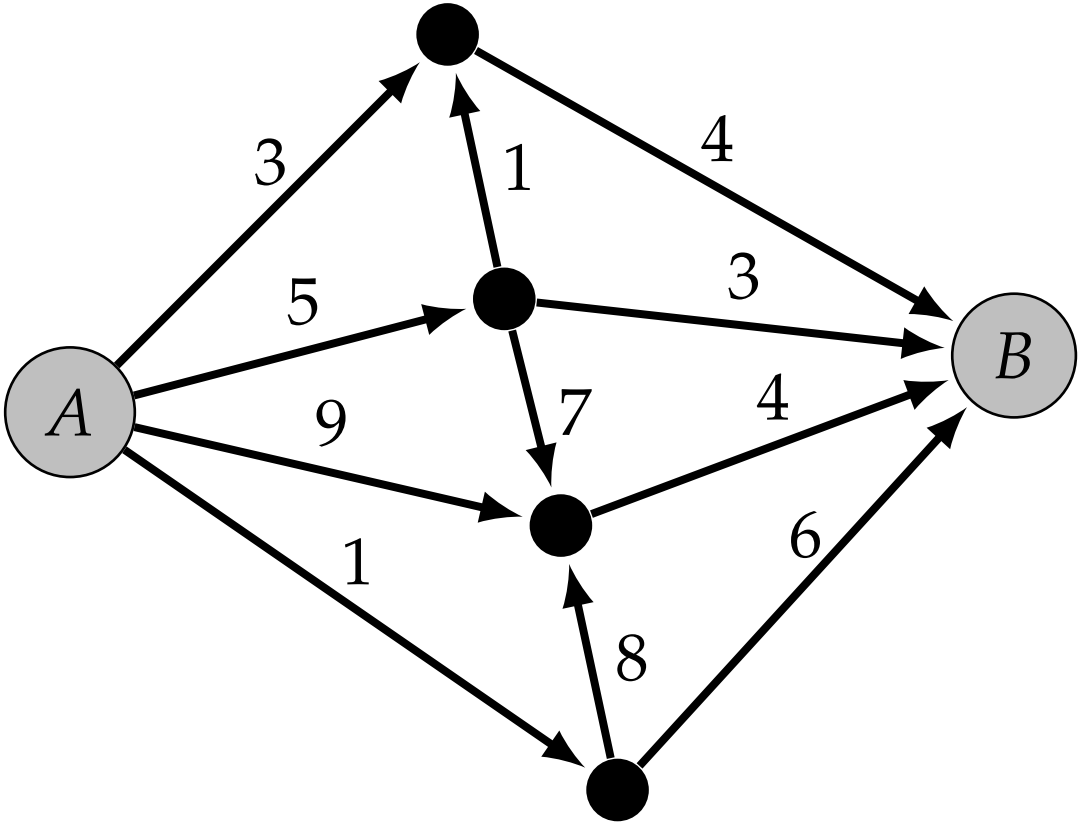
\includegraphics[width=0.2\textwidth]{first.png}
          \end{figure}
          Sabendo que Sônico partiu da cidade $A$ até a cidade $B$, qual a diferença entre a maior e a menor quantidade de anéis que ele pode ter coletado?
        \item Dentro de cada uma de duas caixas há uma bola vermelha ou uma bola verde. Na primeira caixa, do lado de fora, há um aviso:
          ``Dentro de pelo menos uma das duas caixas há uma bola verde'' e na segunda caixa há o aviso: ``Há uma bola vermelha dentro da outra 
          caixa''. Sabe-se que os dois avisos são ambos falsos ou ambos são verdadeiros. O que pode ser afirmado com certeza?
        \item Qual é a soma dos primeiros $2022$ dígitos após a vírgula na representação decimal da fração $\dfrac{2021}{148}$?
        \item Uma data é especial quando ocorre no dia $k$ do mês $k$ e cai no $k$-ésimo dia da semana (em que o primeiro dia da semana é 
          domingo) para algum $k$, $1 \le k \le 7$. Por exemplo, 5 de maio de 2022 é especial, pois caiu na quinta-feira (nesse exemplo, $k=5$).
          Qual é a maior quantidade de dias especiais que pode ocorrer em um ano? \\

          \textit{Dados: Janeiro, Março e Maio têm 31 dias; Fevereiro tem 28 ou 29 dias; Abril e Junho têm 30 dias.} 
        \item A soma dos algarismos do número
          \[
            20222022^2 + 20222021^2 - 2 \times 20222020 \times 20222019
          \]
          é igual a o que?
        \item Na figura, $AD$ é altura e $O$ é o centro da circunferência circunscrita ao triângulo $ABC$. Sabendo que $\angle BAC = 72^\circ$, qual é a medida do ângulo $\angle AEB$?
          
          \begin{figure}[h]
            \centering
            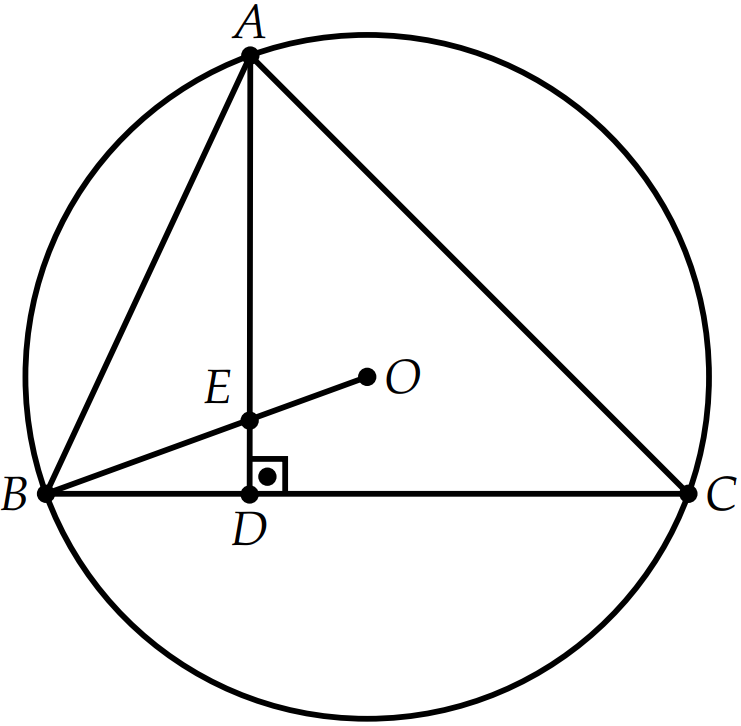
\includegraphics[width=0.2\textwidth]{second.png}
          \end{figure}

          \item Um número inteiro positivo $n$ é tal que:
            \begin{itemize}[nosep]
              \item $n$ possui exatamente $15$ divisores positivos;
              \item $n$ não é múltiplo de $5$.
            \end{itemize}
            Qual é a diferença entre o quarto e o terceiro menores valores possíveis de $n$?
          \item No triângulo $ABC$, retângulo em $A$, temos $AB=6$ e $AC=8$. Seja $D$ o pé da altura relativa ao lado $BC$ e $M$ o ponto médio
            de $BC$. Qual o valor de $DM$?
          \item As raízes da equação $x^{2}-nx+m=0$ são os números reais não nulos $a$ e $b$. As raízes da equação $x^{2}-2nx+2m=0$ são 
            $a^{2}$ e $b^{2}$. Quanto vale $m+n$?
            \item De quantas maneiras podemos cobrir algumas casas de um tabuleiro $10\times 10$ com dominós $2\times 1$ ou $1\times 2$ de tal forma que, dadas quaisquer quatro casas do tabuleiro que compartilham um vértice, exatamente duas delas estão cobertas por dominós? A seguir exibimos parte de um tabuleiro válido, em que os retângulos cinzas representam os dominós.
              \begin{figure}[h]
                \centering
                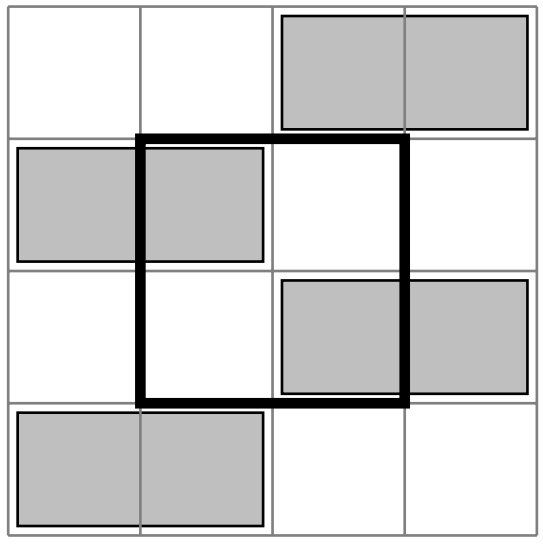
\includegraphics[width=0.2\textwidth]{third.png}
              \end{figure}
      \end{enumerate}
    \subsection{Respostas Numéricas}
    \begin{enumerate}[label=\textbf{\arabic*.}]
              \item Maria observou que os ponteiros de um relógio analógico formavam um ângulo de $33^\circ$ (sim, Maria mediu), como mostra a figura
        a seguir. Após algum tempo, menor do que uma hora, o ponteiro dos minutos (ponteiro maior) passou pelo ponteiro das horas (ponteiro
        menor) e formou novamente um ângulo de $33^\circ$. Quantos minutos se passaram? \\
        \begin{figure}[h]
          \centering
          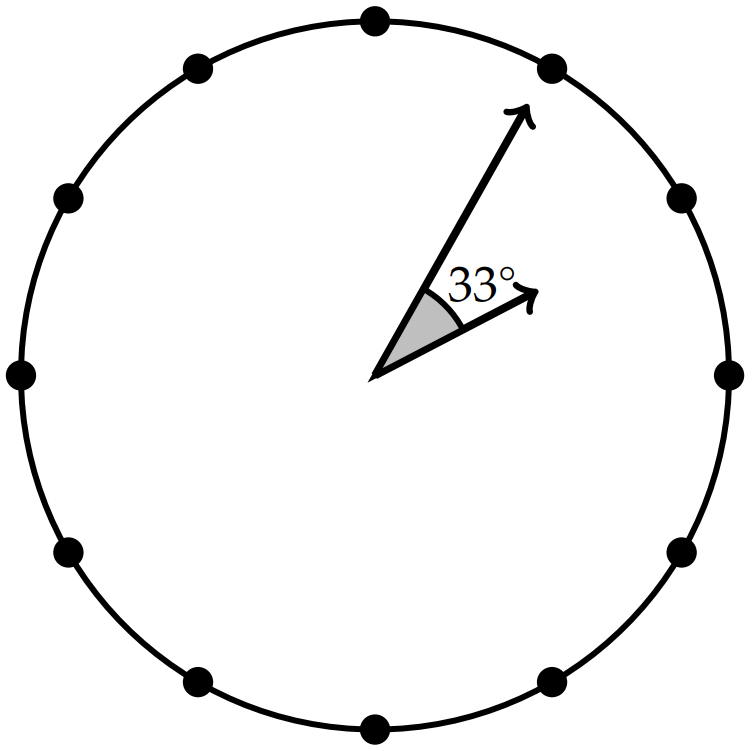
\includegraphics[width=0.2\textwidth]{fourth.png}
        \end{figure}

      \item A calculadora do professor Piraldo tem só um botão. Ao apertá-lo, ele subtrai do número $N$ no visor o seu maior divisor diferente
        de $N$. Por exemplo, se no visor aparece $75$, o botão faz aparecer o número $75-25=50$. Suponha que a calculadora exiba o número
        $5^{2022}$ (a calculadora é bem grande!). Quantas vezes o botão deve ser apertado até que apareça $1$ no visor pela primeira vez?

      \item As 9 casinhas de um tabuleiro $3 \times 3$ devem ser preenchidas com os números de $1$ a $9$, com um número em cada casinha. Um preenchimento é \emph{sinuoso} quando todos os pares de números consecutivos ocupam casas vizinhas (com um lado em comum). O tabuleiro a seguir, por exemplo, é sinuoso:
        \[
          \begin{array}{|c|c|c|}\hline
            1 & 2 & 9 \\ \hline
            4 & 3 & 8 \\ \hline
            5 & 6 & 7 \\ \hline
          \end{array}
        \]
        Quantos são os tabuleiros sinuosos?

      \item Na figura, $M$ é ponto médio do lado de um quadrado de área $36$. Qual é a área do triângulo retângulo cinza? \\
        \begin{figure}[h]
          \centering
          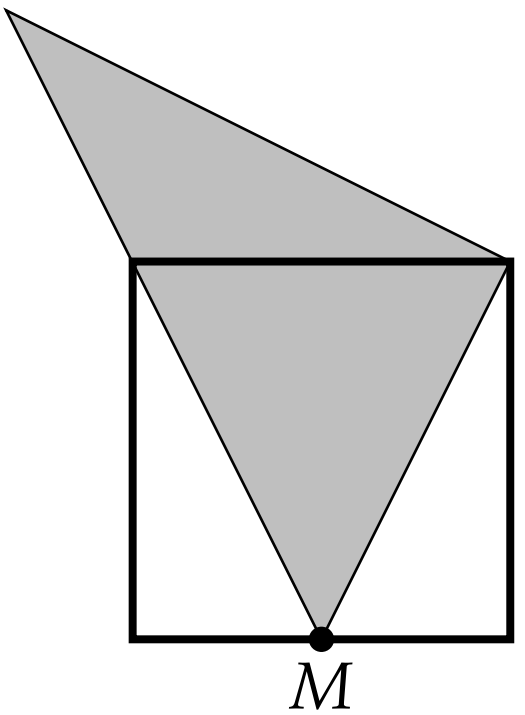
\includegraphics[width=0.2\textwidth]{fifth.png}
        \end{figure}

      \item Para cada $x$ real denotamos $\kb{x}$ o maior inteiro menor que ou igual a $x$. Por exemplo, $\kb{3{,}15}=3$. Sabendo que
        \[
          \kb{\sqrt{1}}+\kb{\sqrt{2}}+\kb{\sqrt{3}}+\cdots+\kb{\sqrt{n}}=217,
        \]
        qual é o valor de $n$? \\

      \end{enumerate}

  \clearpage

  \section{\textsf{Soluções}}
    \subsection{Problema 1}
      \begin{tcolorbox}[statementbox]
        Sônico, o tatu bola veloz, está caminhando pelas estradas do planeta Mobius coletando anéis. Abaixo está um mapa com a
        quantidade de anéis em cada estrada do reino. Sabendo que Sônico partiu da cidade $A$ até a cidade $B$, a diferença entre a maior
        e a menor quantidade de anéis que ele pode ter coletado é:
        \begin{center}
          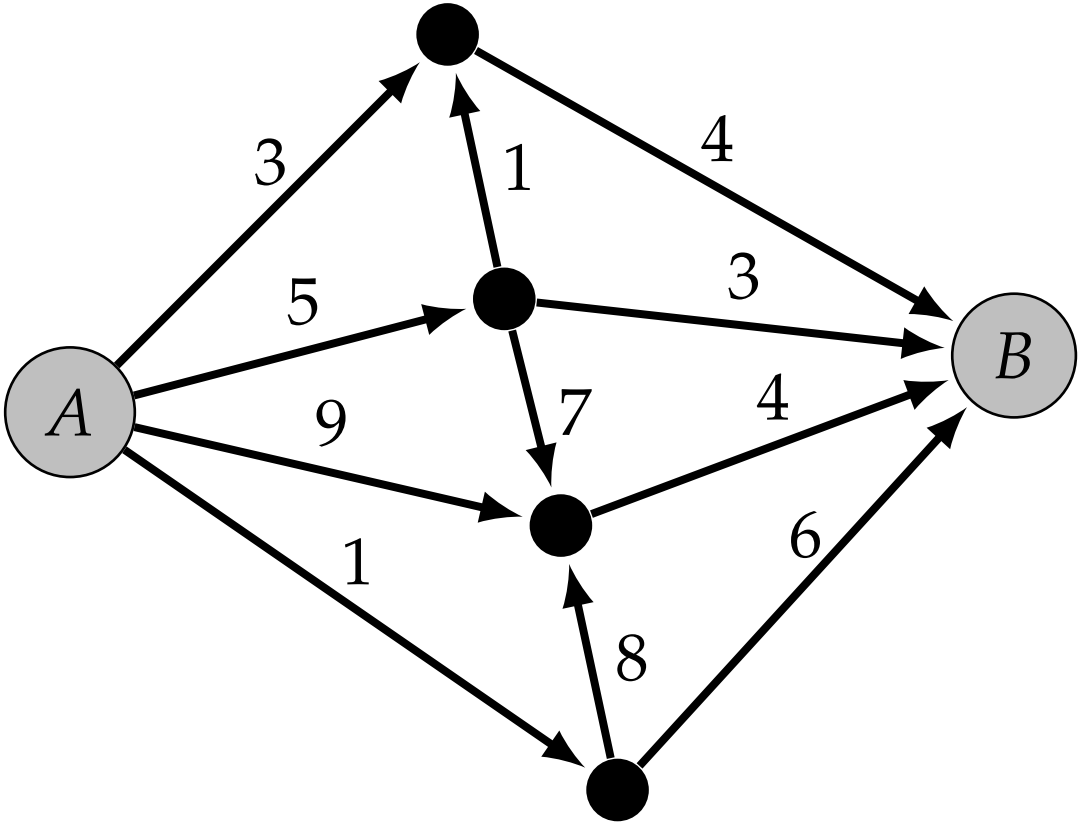
\includegraphics[width=0.25\textwidth]{first.png}
        \end{center}
      \end{tcolorbox}


    \clearpage

    \subsection{Problema 2}
      \begin{tcolorbox}[statementbox]
        Dentro de cada uma de duas caixas há uma bola vermelha ou uma bola verde. Na primeira caixa, do lado de fora, há um aviso:
        `Dentro de pelo menos uma das duas caixas há uma bola verde'' e na segunda caixa há o aviso: `Há uma bola vermelha dentro da outra
        caixa''. Sabe-se que os dois avisos são ambos falsos ou ambos são verdadeiros. O que pode ser afirmado com certeza?
      \end{tcolorbox}

    \clearpage

    \subsection{Problema 3}
      \begin{tcolorbox}[statementbox]
        Qual é a soma dos primeiros $2022$ dígitos após a vírgula na representação decimal da fração $\frac{2021}{148}$
      \end{tcolorbox}

    \clearpage

    \subsection{Problema 4}
      \begin{tcolorbox}[statementbox]
        Uma data é especial quando ocorre no dia $k$ do mês $k$ e cai no $k$-ésimo dia da semana (em que o primeiro dia da semana é 
        domingo) para algum $k$, $1 \le k \le 7$. Por exemplo, 5 de maio de 2022 é especial, pois caiu na quinta-feira (nesse exemplo, $k=5$).
        Qual é a maior quantidade de dias especiais que pode ocorrer em um ano? \\
        \textit{Dados:} Janeiro, Março e Maio têm 31 dias; Fevereiro tem 28 ou 29 dias; Abril e Junho têm 30 dias.
      \end{tcolorbox}

    \clearpage

    \subsection{Problema 5}
      \begin{tcolorbox}[statementbox]
        A soma dos algarismos do número
        \[
          20222022^2 + 20222021^2 - 2 \times 20222020 \times 20222019
        \]
        é igual a
      \end{tcolorbox}

    \clearpage

    \subsection{Problema 6}
\begin{tcolorbox}[statementbox]
Na figura, $AD$ é altura e $O$ é o centro da circunferência circunscrita ao triângulo $ABC$. Sabendo que $\angle BAC = 72^\circ$, qual é a medida do ângulo $\angle AEB$?

\begin{center}
  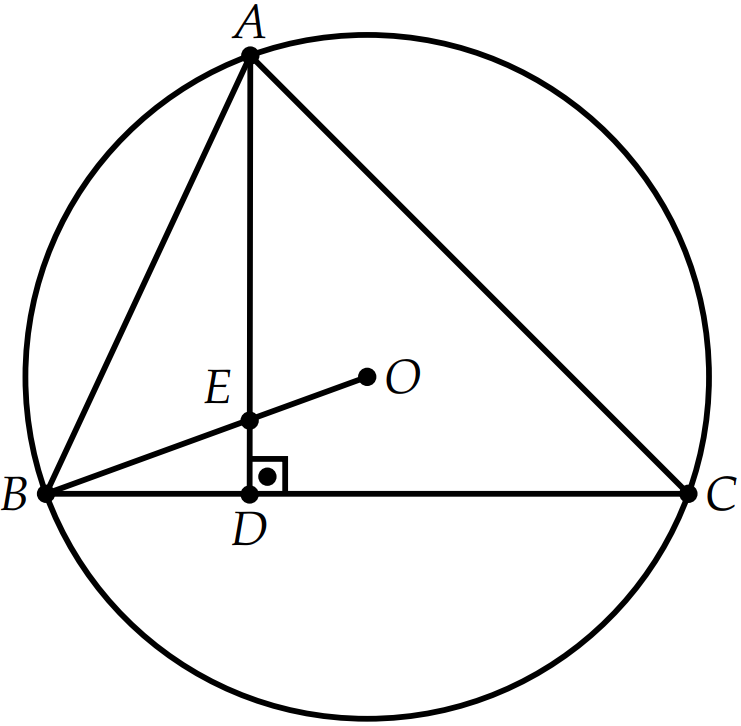
\includegraphics[width=0.23\textwidth]{second.png}
\end{center}
\end{tcolorbox}

\clearpage

\subsection{Problema 7}
\begin{tcolorbox}[statementbox]
Um número inteiro positivo $n$ é tal que:
\begin{itemize}[nosep]
  \item $n$ possui exatamente $15$ divisores positivos;
  \item $n$ não é múltiplo de $5$.
\end{itemize}
Qual é a diferença entre o quarto e o terceiro menores valores possíveis de $n$?
\end{tcolorbox}

\clearpage

\subsection{Problema 8}
\begin{tcolorbox}[statementbox]
No triângulo $ABC$, retângulo em $A$, temos $AB=6$ e $AC=8$. Seja $D$ o pé da altura relativa ao lado $BC$ e $M$ o ponto médio
de $BC$. O valor de $DM$ é
\end{tcolorbox}

\clearpage

\subsection{Problema 9}
\begin{tcolorbox}[statementbox]
As raízes da equação $x^{2}-nx+m=0$ são os números reais não nulos $a$ e $b$. As raízes da equação $x^{2}-2nx+2m=0$ são 
$a^{2}$ e $b^{2}$. O valor de $m+n$ é
\end{tcolorbox}

\clearpage

\subsection{Problema 10}
\begin{tcolorbox}[statementbox]
De quantas maneiras podemos cobrir algumas casas de um tabuleiro $10\times 10$ com dominós $2\times 1$ ou $1\times 2$ de tal forma que, dadas quaisquer quatro casas do tabuleiro que compartilham um vértice, exatamente duas delas estão cobertas por dominós? A seguir exibimos parte de um tabuleiro válido, em que os retângulos cinzas representam os dominós.
\begin{center}
  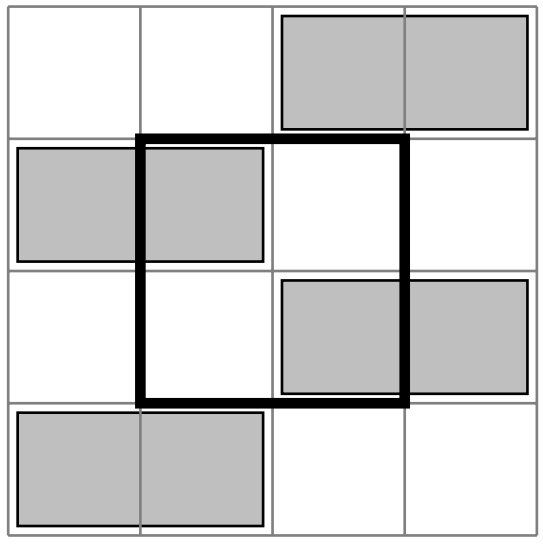
\includegraphics[width=0.2\textwidth]{third.png}
\end{center}
\end{tcolorbox}

\clearpage

\subsection{Problema 11}
\begin{tcolorbox}[statementbox]
Maria observou que os ponteiros de um relógio analógico formavam um ângulo de $33^\circ$ (sim, Maria mediu), como mostra a figura
a seguir. Após algum tempo, menor do que uma hora, o ponteiro dos minutos (ponteiro maior) passou pelo ponteiro das horas (ponteiro
menor) e formou novamente um ângulo de $33^\circ$. Quantos minutos se passaram? \\
\begin{center}
  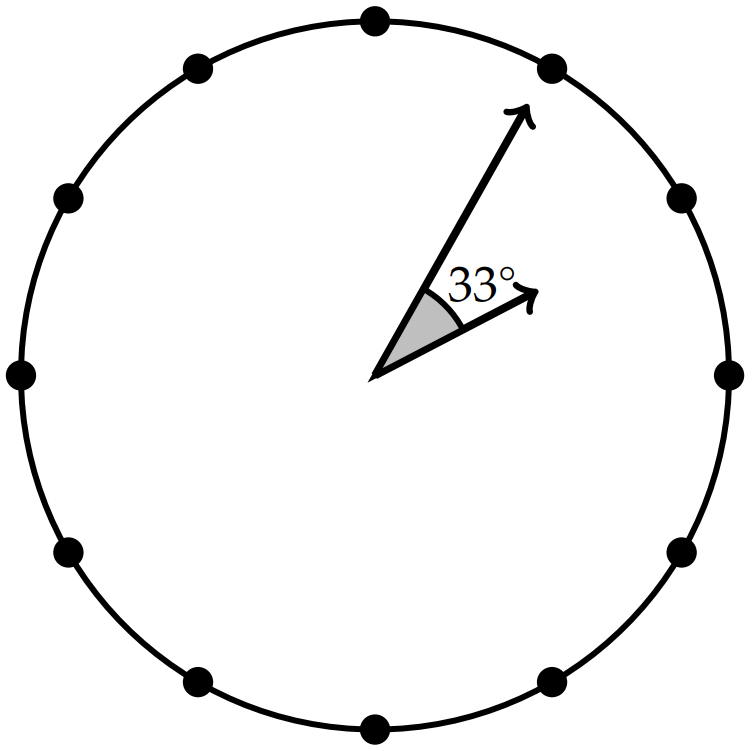
\includegraphics[width=0.2\textwidth]{fourth.png}
\end{center}
\end{tcolorbox}

\clearpage

\subsection{Problema 12}
\begin{tcolorbox}[statementbox]
A calculadora do professor Piraldo tem só um botão. Ao apertá-lo, ele subtrai do número $N$ no visor o seu maior divisor diferente
de $N$. Por exemplo, se no visor aparece $75$, o botão faz aparecer o número $75-25=50$. Suponha que a calculadora exiba o número
$5^{2022}$ (a calculadora é bem grande!). Quantas vezes o botão deve ser apertado até que apareça $1$ no visor pela primeira vez?
\end{tcolorbox}

\clearpage

\subsection{Problema 13}
\begin{tcolorbox}[statementbox]
As 9 casinhas de um tabuleiro $3 \times 3$ devem ser preenchidas com os números de $1$ a $9$, com um número em cada casinha. Um preenchimento é \emph{sinuoso} quando todos os pares de números consecutivos ocupam casas vizinhas (com um lado em comum). O tabuleiro a seguir, por exemplo, é sinuoso:
\[
  \begin{array}{|c|c|c|}\hline
    1 & 2 & 9 \\ \hline
    4 & 3 & 8 \\ \hline
    5 & 6 & 7 \\ \hline
  \end{array}
\]
Quantos são os tabuleiros sinuosos?
\end{tcolorbox}

\clearpage

\subsection{Problema 14}
\begin{tcolorbox}[statementbox]
Na figura, $M$ é ponto médio do lado de um quadrado de área $36$. Qual é a área do triângulo retângulo cinza? \\
\begin{center}
  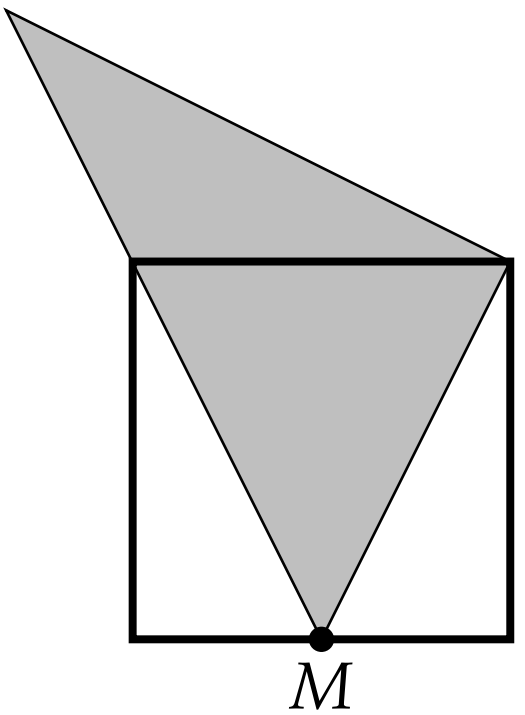
\includegraphics[width=0.2\textwidth]{fifth.png}
\end{center}
\end{tcolorbox}

\clearpage

\subsection{Problema 15}
\begin{tcolorbox}[statementbox]
Para cada $x$ real denotamos $\kb{x}$ o maior inteiro menor que ou igual a $x$. Por exemplo, $\kb{3{,}15}=3$. Sabendo que
\[
  \kb{\sqrt{1}}+\kb{\sqrt{2}}+\kb{\sqrt{3}}+\cdots+\kb{\sqrt{n}}=217,
\]
qual é o valor de $n$? \\
\end{tcolorbox}

  \clearpage

  \section{\textsf{Referências}}
\end{document}
